\documentclass[pdflatex,sn-basic,Numbered]{sn-jnl}

\usepackage{graphicx}
\usepackage{multirow}
\usepackage{amsmath,amssymb,amsfonts}
\usepackage{amsthm}
\usepackage{mathrsfs}
\usepackage[title]{appendix}
\usepackage{xcolor}
\usepackage{textcomp}
\usepackage{manyfoot}
\usepackage{booktabs}
\usepackage{algorithm}
\usepackage{algorithmicx}
\usepackage{algpseudocode}
\usepackage{listings}

\raggedbottom

\begin{document}

\title[Unsupervised Functional Stage Detection From EEG Using Topological Data Analysis]{Unsupervised Functional Stage Detection From EEG Using Topological Data Analysis}

\author*[1]{\fnm{Aleksandr} \sur{Abramov}}\email{asabramov@edu.hse.ru}
\author[1]{\fnm{Ekaterina} \sur{Mikhaylets}}
\author[2]{\fnm{Vsevolod} \sur{Chernyshev}}
\author[3]{\fnm{Alexander} \sur{Kaplan}}
\author[1]{\fnm{Fedor} \sur{Ratnikov}}

\affil[1]{\orgdiv{Faculty of Computer Science}, \orgname{HSE University}, \orgaddress{\state{Moscow}, \country{Russia}}}
\affil[2]{\orgname{Ulm University}, \orgaddress{\state{Ulm}, \country{Germany}}}
\affil[3]{\orgname{Lomonosov Moscow State University}, \orgaddress{\state{Moscow}, \country{Russia}}}

\abstract{Electroencephalogram (EEG) segmentation is is still largely performed manually by specialists. Recent studies have proposed the state-detecting algorithm (SDA) --- an automated technique for detecting functional stages with minimal human intervention --- which has proven effective using spectral features. This paper introduces an alternative feature engineering approach that explores the spatial structure of data using the emerging field of topological data analysis (TDA). We propose an algorithm to extract a comprehensive topological description of EEG with tens of thousands of features and introduce the quick state-detecting algorithm (QSDA), a feature selection framework based on SDA performance. Next, we apply the procedure to EEG recordings from two distinct domains --- Guhyasamaja Tantra meditation and whole-night polysomnographic sleep --- and observe well-separated stage boundaries across most recordings, suggesting that TDA may complement or outperform spectral features in some settings. We also observed encouraging performance on noisy data, whereas shuffled epochs produced substantially weaker boundaries, supporting the robustness of the technique within the settings examined. Overall, the algorithm appears to be a promising feature engineering approach for SDA and suggests that the spatial structure of EEG may contain informative patterns. These findings motivate further investigation of their possible physiological interpretation, as well as an assessment across broader EEG paradigms.}

\keywords{topological data analysis, state-detecting algorithm, functional states, feature selection}

\maketitle

\section{Introduction}

Electroencephalograms (EEG) are a powerful tool for studying human brain activity and diagnosing numerous diseases and abnormalities. However, EEG analysis is still often performed manually, and automation in the field is largely limited to specific tasks. Most algorithms rely on information about events artificially created during the experiment (external interactions with the subject, reactions, responses, etc.). Currently, the study of EEG recorded during continuous processes that do not allow external interactions with the subject is of significant value for neurophysiology, including somnology and, potentially, epilepsy detection.

One such task is to find the boundaries of functional states in the EEG that split the recording into well-separable parts, denoting the occurrence of some naturally induced events. Due to the very domain-specific nature and size of the dataset, the popular modern methods, including transformers and diffusion learning~\cite{AGHAYENGEJEH2025100792,POURHAJIAGHAYENGEJEH2026114975}, are not applicable. To solve this problem,~\cite{SDA} recently presented the state-detecting algorithm (SDA), which operates without any additional information about the events that occurred during the experiment (including their count) using traditional data clustering methods. To use the algorithm, one should clean and preprocess the EEG data, split it into epochs, and embed the corresponding time series into some feature space. As shown in the original work, the method performed well for EEG obtained from the Tantric Guhyasamaja meditation of Buddhist monks using traditional spectral features to describe the time series: PSD, PLV, and Coherence.

However, these features mostly describe the frequencies and correlations in the time series, leaving significant portions of the information unexplored. Currently, there is ongoing research on the applications of another modern approach to feature extraction --- topological data analysis (TDA), which identifies the relationships in the data by studying its geometry and spatial structure based on the appearance and disappearance of holes and voids across dimensions. It enables quantification of structural characteristics of the signal that may be informative for physiological applications, can improve performance in some tasks, and may offer interpretable representations.

Numerous recent studies have shown that TDA demonstrates high quality in solving various problems, including time series and EEG in particular. For example,~\cite{chazal2024topologicalanalysisdetectinganomalies,rai2024identifyingextremeeventsstock,heo2024persistenthomologyfeaturedtime,chrétien2024timetopologicalanalysiseeg} presented numerous theoretically guaranteed approaches to detecting anomalies in multivariate time series, demonstrating their quality with diverse datasets ranging from synthetic ones to real-world examples, including the stock market, music recordings, and epilepsy detection.~\cite{cai2024topologicalfeaturesearchmethod} demonstrated the application of TDA in ADHD classification, achieving exceptional results for typical datasets in the field. Finally,~\cite{deng2024twostagehierarchicalexplainablefeature} suggested a TDA-based feature selection framework to improve the performance of dimensionality reduction in sleep stage classification.

Despite this breadth of applications, as reviewed in~\cite{10.3389/fnins.2021.761703}, TDA-based EEG studies have operated predominantly in supervised settings with labeled data. To the best of our knowledge, among the studies reviewed, no prior work has evaluated the approach in an unsupervised segmentation framework or compared it against spectral methods across fundamentally different EEG paradigms. This paper addresses both gaps.

In this study, we apply topological data analysis to find functional states in the EEG of continuous processes --- the aforementioned Tantric Guhyasamaja meditation practice and whole-night polysomnographic sleep recordings (PSG). To evaluate the applicability of the approach to the problem, we propose a framework for calculating a comprehensive description with tens of thousands of features describing various aspects of the time series using diverse topological methods and statistical characteristics. We then present QSDA, an SDA-based technique to select a reasonable number of features with the best quality. We show that the approach effectively filters out the least valuable features and can noticeably improve the results. Finally, we compare the obtained state boundaries with expert annotations for sleep data and with results obtained using different feature sets and data modifications for meditation data, and draw conclusions based on the output's quality metrics. Additionally, we utilize information value analysis (IV) to estimate the influence of individual features on the answer, confirm the stability of our algorithm, and reinforce the obtained results.

\section{Methods}

\subsection{Datasets}

\subsubsection{Meditation data}

Guhyasamaja Tantra is a traditional meditation practice that follows the strict principles enshrined in the sacred scriptures of Buddhism. Its essential part consists of eight sequential stages, the durations of which may vary in different versions.

The data used in the study are EEG recordings of the successful meditation of 30 Tibetan Buddhist monks practicing Guhyasamaja Tantra for many decades. The dataset was collected during three expeditions, each of which yielded recordings from 12, 14, and 4 monks, respectively. The signals were acquired using an NVX-52 system at a 500 Hz sampling rate with analog bandpass filtering from 0.1 to 200 Hz and a digital notch filter at 50 Hz to remove power line noise. The first three recordings have been presented in the original paper~\cite{SDA}, and are thus of the most interest in this work. 

Several procedures, including a bandpass filter at 0.9--40 Hz and independent component analysis, were applied to remove artifacts unrelated to the process of interest (respiratory and muscle activity, eye blinking, heartbeat, etc.). The recordings were then divided into 1-second epochs and, before any subsequent analysis, we discarded 10--15\% of epochs most deviating from the average by the power spectral density computed using the adaptive multitaper method. Please refer to the original study~\cite{SDA} for further details and parameters of the preprocessing pipeline.

Since the recordings were obtained during separate expeditions, the dataset includes three groups of EEG with slightly different electrode sets. The first expedition (12 recordings) used 38 electrodes, whereas the second (14 recordings) and third (4 recordings) utilized only 32, differing in the placement of AF1, AF2, F3, and F4. In all cases, ear electrodes were excluded from analysis, as their data primarily describe muscular activity, which is irrelevant to the study. As in the original paper, we divided the electrodes into 11 regions of interest based on the scalp regions, as shown in Supplementary Materials A:\@ pre-frontal (FP), left frontal (LF), midline frontal (MF), right frontal (RF), left central (LC), midline central (MC), right central (RC), left temporal (LT), right temporal (RT), parietal (PAR), and occipital (OCC).

\subsubsection{Sleep data}

To validate the approach and assess its general applicability, we rely on Sleep-EDF~\cite{SleepEdf,PhysioNet} --- a more common, public dataset of 197 whole-night polysomnographic sleep recordings. It contains two subsets: 153 recordings from the Sleep Cassette Study (SC) and 44 recordings from the Sleep Telemetry Study (ST). In this paper, we focus on healthy aging and therefore use the former group, while excluding the ST subset as it contains recordings from patients with known sleep disorders or under medication.

The data were obtained during a 1987--1991 study of age effects on sleep involving 77 subjects aged between 25 and 101. In this study, though, we discard any additional information about the subjects, including their age and sex, and focus on the PSG recordings themselves. The signals contain three EEG channels, one EOG channel, chin EMG, body temperature, and a respiration monitoring channel. For each recording, the dataset also provides stage annotations from well-trained experts. To speed up the computations, we resample all channels from 100 Hz to 50 Hz, crop the data to a maximum of 15 minutes of wake time at the beginning and end of the recording, and split it into 15-second and 30-second epochs without overlapping. To simplify the analysis, we also discard the segments with unknown labels, combine stages N3 and N4, and predict at most 10 sleep stages for each subject to compare them with the best-fit subset of 10 stages from the target annotation.


\subsection{State-Detecting algorithm}

The State-Detecting algorithm is a novel data-driven approach for finding the functional states in the EEG from its feature description --- a matrix that maps each epoch to a feature vector of a given dimension. The technique combines two clustering methods to find the resulting edges, accounting for the continuity of the process under analysis in time. Here, we briefly review the general principles of both stages. Please refer to the original study~\cite{SDA} for a more detailed description.

In the first step, the algorithm finds the potential boundaries of functional states using Ward's hierarchical clustering method with different values for the number of sought stages and the maximum time between epochs in the connectivity matrix. The obtained boundaries are then sorted, and the neighboring stages are merged if they are too short or do not differ sufficiently by the Ward distance.

In the second step, the algorithm utilizes K-Means to select the candidates for the final boundaries based on the results of the first step. For this, SDA applies the aforementioned clustering method to the joint sets of potential boundaries obtained previously and determines the required number of stages. Finally, the algorithm computes the resulting boundaries as modes and medians of the obtained clusters merged similarly to the first stage to guarantee their sufficient length and dissimilarity.

The definitive answer is selected manually by an expert based on the clustering quality metrics. In this study, we focus on the silhouette score ranging from $-1$ to $1$, with positive values indicating that the object is assigned to the correct cluster, well separated from other clusters. Since the same stage may recur in a recording, we use the so-called adapted silhouette computed as the average score over all pairs of adjacent clusters, thus measuring local separation and being unaffected by distant recurrences of the same label.

\subsection{Topological data analysis}

Topological data analysis is a modern approach to analyzing different data by studying their spatial characteristics (shape, structure, etc.) using algebraic topology. The main tools of this approach are persistent homology and persistence diagrams, calculated for metric spaces to describe the number and stability of multidimensional `holes' in them. Previous studies have shown that minor perturbations in the source data do not significantly affect the results. This stability makes persistence diagrams useful for machine learning according to the following general pipeline.

First, one should transform the input data into a metric space --- a set of points with a correctly defined distance function. In this study, we utilized two principal approaches: the Takens' embedding algorithm~\cite{10.1007/BFb0091924,perea2013slidingwindowspersistenceapplication} to explore individual components of the time series and the Pearson dissimilarity to investigate correlations between them. For the former, we adjust two primary hyperparameters: the time delay and the embedding dimension. Typical selection methods aim to optimize the mutual information~\cite{PhysRevA.33.1134} and the number of false-neighboring pairs of points~\cite{PhysRevA.45.3403} respectively. For the latter, we define the distances between the components of a multivariate time series as their Pearson dissimilarity, thus obtaining a point cloud.

Second, we construct a sequence of nested simplicial complexes. These are topological spaces homotopy equivalent to unions of balls of increasing radius around the points in the set. However, due to excessive computational costs, in practice, an approximation called the Vietoris---Rips complex~\cite{Vietoris1927} is typically utilized. The structure is built from simplices --- segments, triangles, tetrahedra, and higher-dimensional analogues. A simplex is included if all pairwise distances between its vertices are less than $\epsilon$. The general algorithm for constructing a filtration is to observe the appearance and disappearance of simplices with increasing values of $\epsilon$, although several more efficient algorithms have been proposed (e.g.~\cite{Bauer_2021}).

Next, one calculates the persistent homology of the resulting structure and constructs a persistence diagram, where each homological feature corresponds to one point with coordinates representing the moments of its appearance in and disappearance from the complex, respectively. Subsequently, we extract the features --- various topological and statistical characteristics --- from the persistence diagram. The principal approach studies Betti numbers~\cite{Zomorodian2005}, which represent the number of independent homology classes. Multiple other techniques have been proposed, including persistence entropy~\cite{10.1007/978-3-319-29228-1_11}, landscape~\cite{bubenik2015statisticaltopologicaldataanalysis}, silhouette~\cite{chazal2013stochasticconvergencepersistencelandscapes}, and amplitudes. The latter are particularly interesting as measures of the difference between a given persistence diagram and an `empty' one. These can be computed based on other topological characteristics or related metrics, such as the Wasserstein and bottleneck distances~\cite{Efrat2001}.

Finally, we select the most valuable features and reduce their dimensionality to remove noise and improve the quality of subsequent machine learning algorithms. For the latter, we used principal component analysis (PCA), which is a typical method that has demonstrated reliability and good performance in many previous studies. As in the original paper, the technique was applied independently to each subject's feature space with 15 components, which preserves 60--80\% of the variance, a common threshold in EEG studies. We further confirm stability of this choice experimentally in Section~\ref{meditation_results}.

\subsection{Feature engineering}

As shown in Fig.~\ref{figure1}, we employ three independent techniques to extract EEG features.

First, the components are processed independently to analyze the data obtained at each electrode separately from other parameters. For this, we divide the epochs --- multidimensional time series --- into sets of one-dimensional time series, each corresponding to one electrode during the experiment. Then, we calculate the optimal hyperparameters of the Takens embedding and acquire a set of values for each epoch of each EEG component. Finally, we select one value for each component that is optimal for most epochs, embed the data into metric spaces using Takens' algorithm with these parameters, construct Vietoris---Rips complexes with simplices of dimensions 1 and 2, and compute persistence diagrams with no limit on the filtration parameter.

This approach describes individual EEG variables and detects most patterns in the data. However, it does not account for correlations between the components, which may also contain valuable information. To address this issue, the second approach aims to analyze the relationships between EEG components. The point clouds are obtained from Pearson dissimilarities between channels, considered as points, across each epoch and its sliding windows, with distances reflecting EEG component correlations. Then, similar to other techniques, we construct Vietoris---Rips complexes up to simplex dimension 5 to produce persistence diagrams and obtain the feature descriptions.\@

Eventually, we analyze the time series as a whole without explicitly focusing on specific characteristics. To do this, we employ the multidimensional Takens algorithm with hyperparameters determined experimentally but kept identical for all components. The retrieved metric spaces are again processed with Vietoris---Rips complexes with simplices of dimensions 1, 2, 3 and an unlimited filtration parameter.

All three branches of the pipeline were implemented with methods available within the giotto-tda Python package~\cite{tauzin2021giottotdatopologicaldataanalysis}.

\subsubsection{Extracting features from persistence diagrams}

To vectorize the persistence diagrams as part of the feature engineering process, we implemented the pipeline in Fig.~\ref{figure2}.

\begin{figure} 
    \centering 
    \begin{minipage}[t]{0.4\textwidth} 
        \vspace{0pt}
        \centering 
        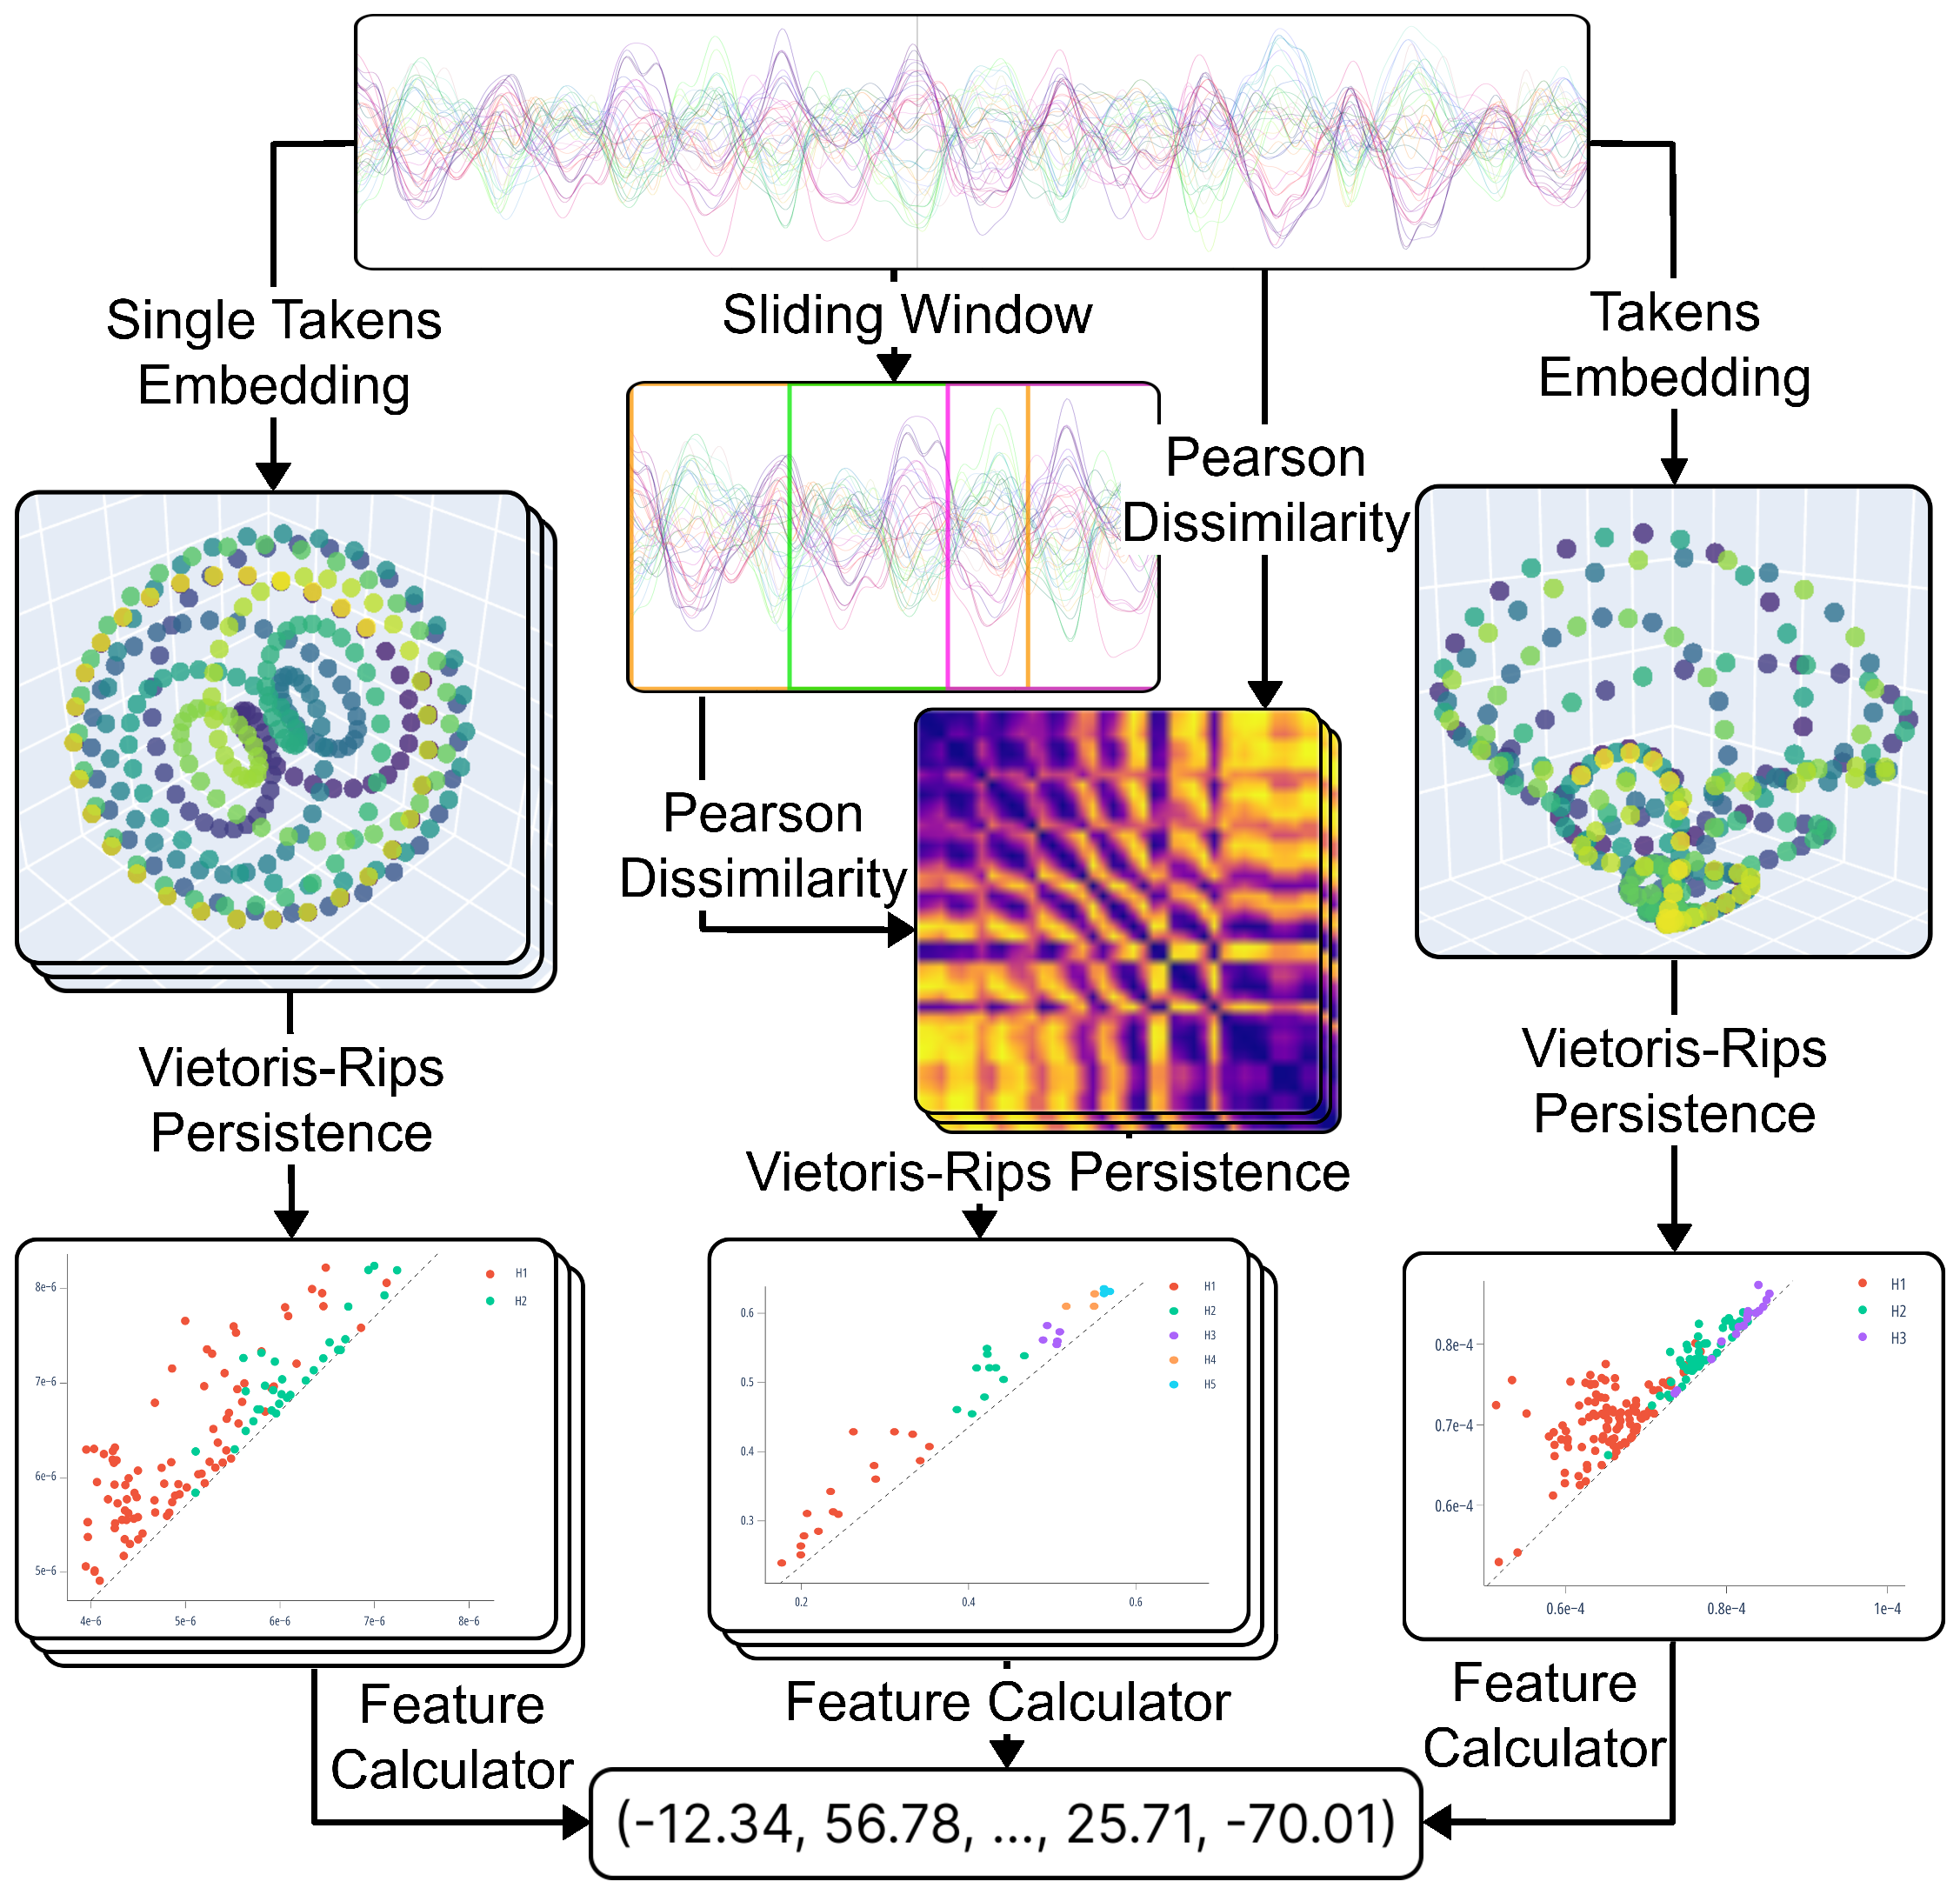
\includegraphics[width=\linewidth]{Fig1.eps} 
        \caption{The algorithm for extracting topological features from the EEG.\@ The last feature calculator step refers to the persistence diagram vectorization pipeline outlined in Fig.~\ref{figure2}\@}\label{figure1} 
    \end{minipage} 
    \hfill 
    \begin{minipage}[t]{0.55\textwidth} 
        \vspace{0pt}
        \centering 
        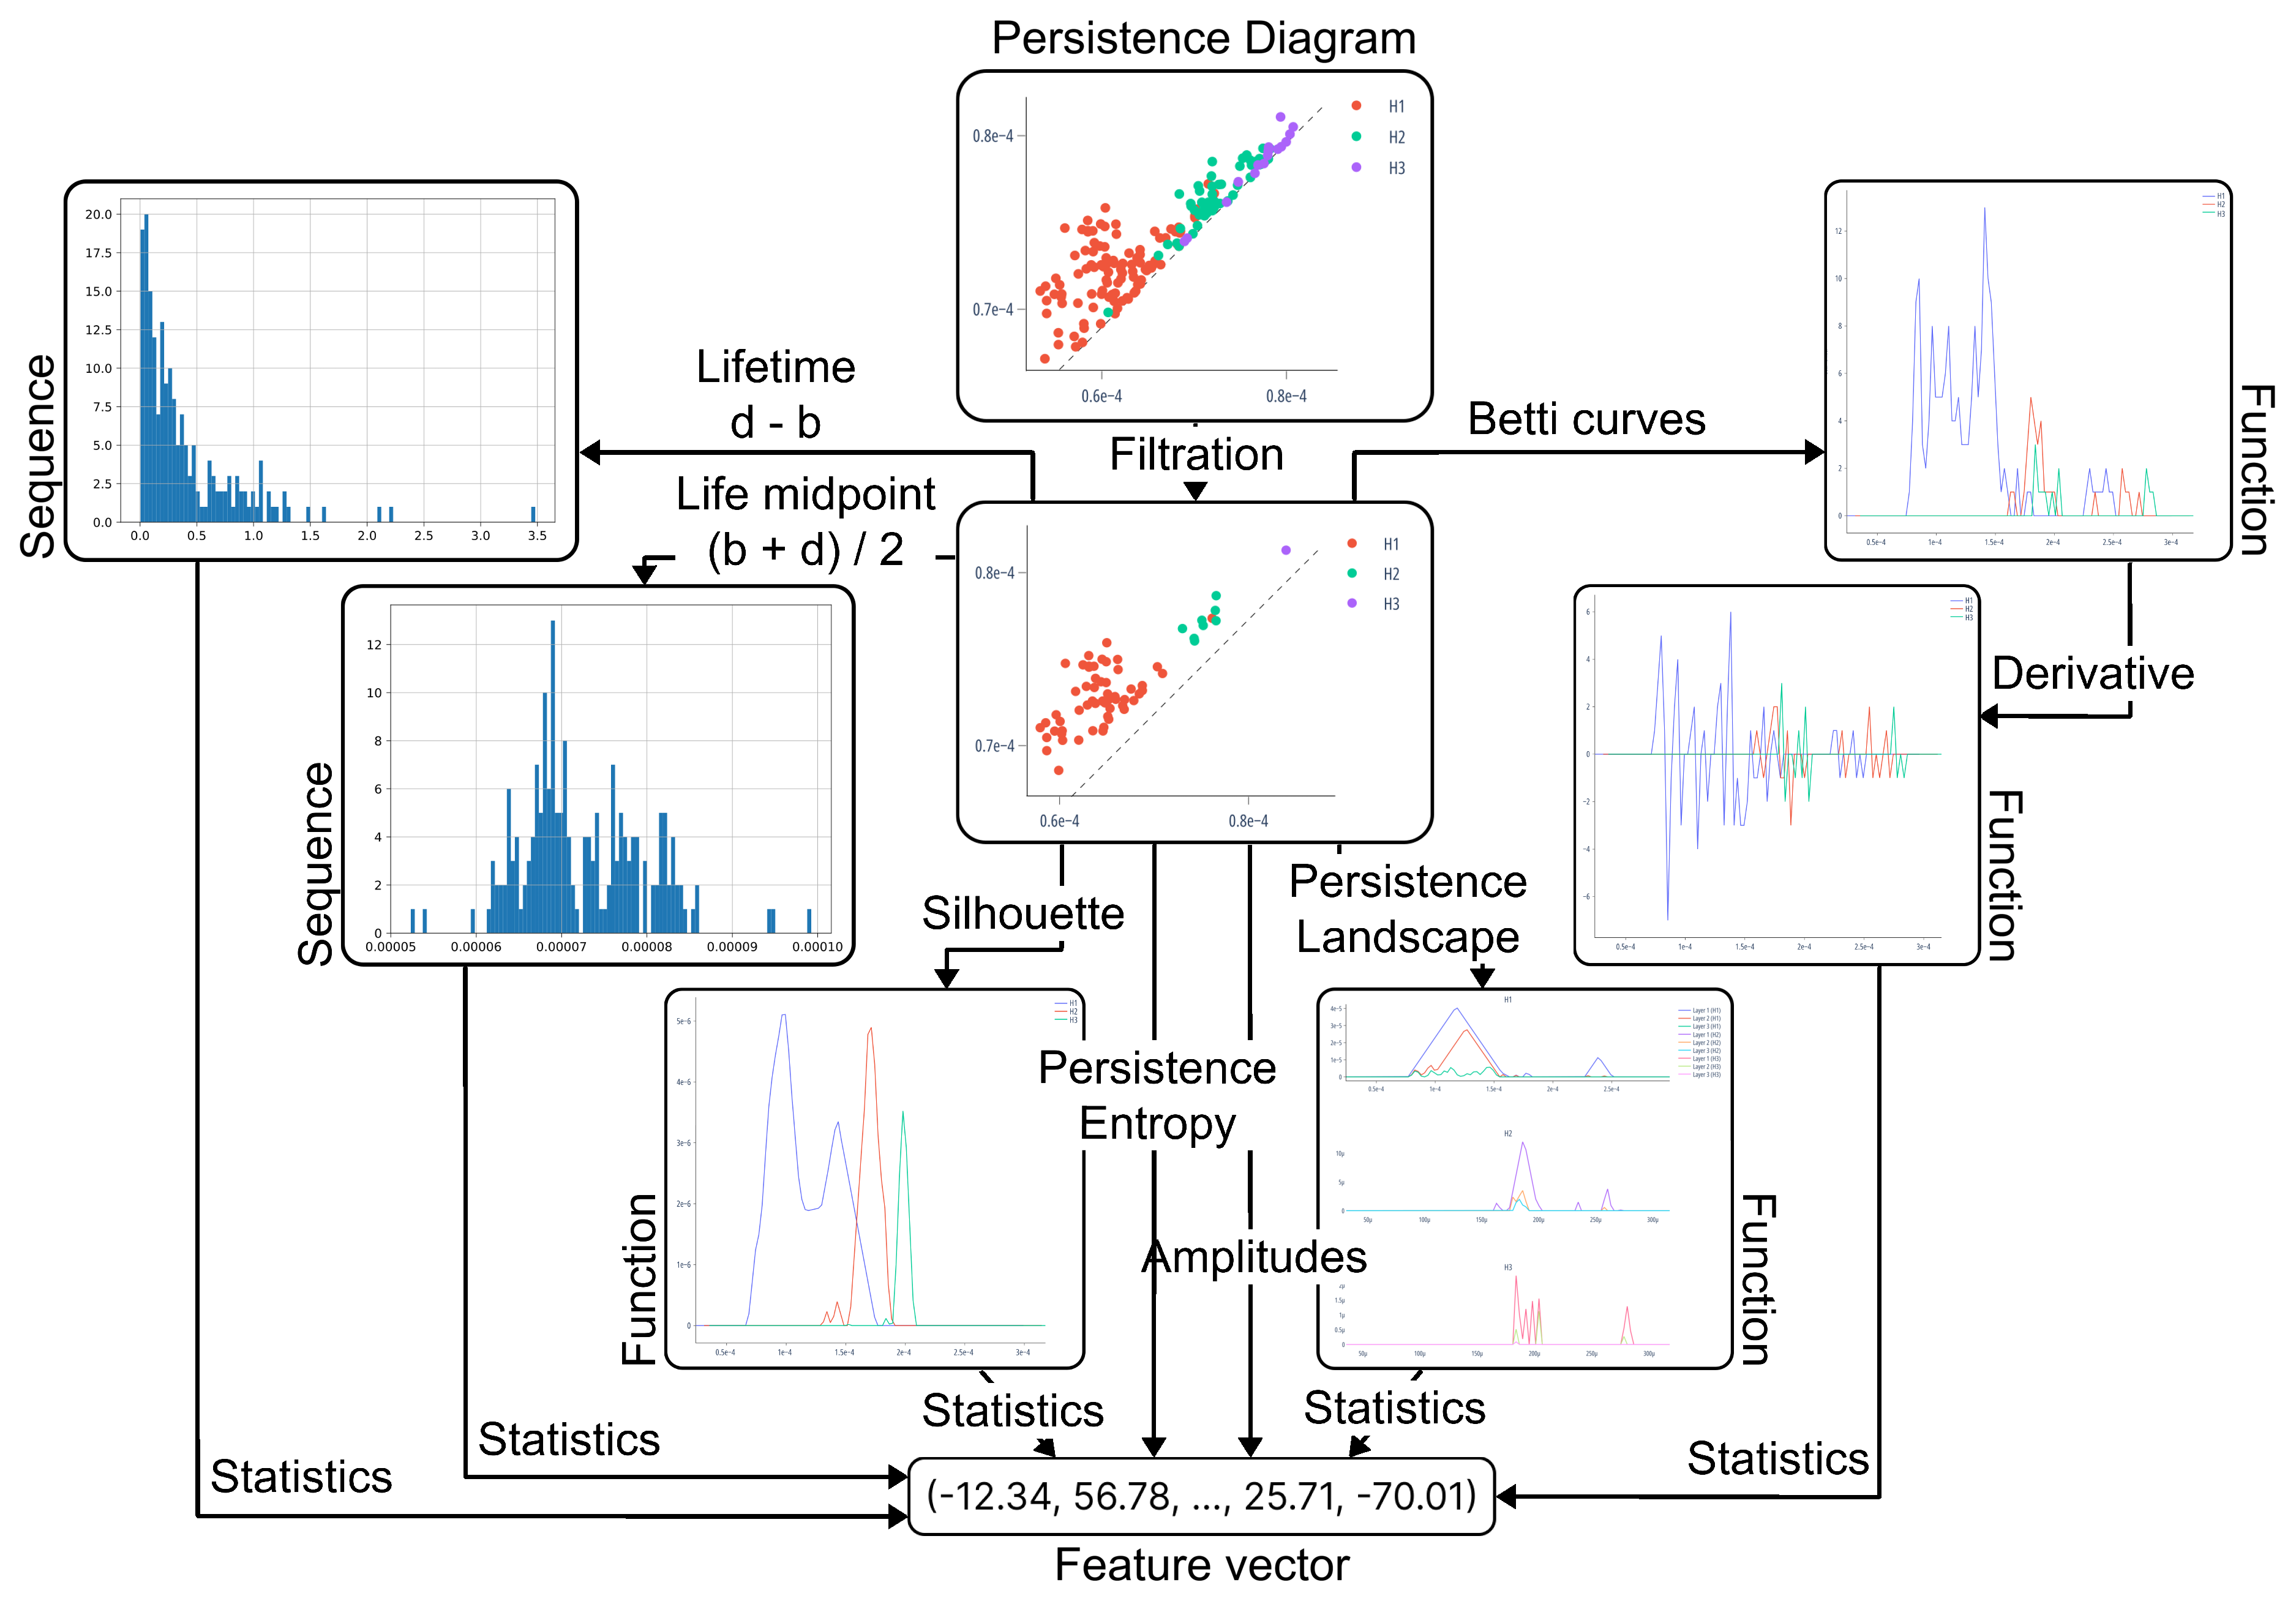
\includegraphics[width=\linewidth]{Fig2.eps} 
        \caption{The pipeline for vectorizing persistence diagrams. For each numeric sequence or function, we extract summary statistics. For functions, we first sample 100 uniformly spaced values over the interval of interest}\label{figure2} 
    \end{minipage} 
\end{figure}

To improve the generalization ability of the features, we first remove a fixed fraction of persistence-diagram points closest to the diagonal, which correspond to the shortest-lived homological features. These points usually carry little information and most likely represent `noise': patterns present in individual recordings but not generic across the objects. The remaining points, in turn, are the most `long-lived' features that are generally most interesting for the analysis.

The algorithm then constructs a comprehensive feature description of the persistence diagram using various topological (persistence landscape, persistence silhouette, amplitudes based on these measures as well as Wasserstein distances) and statistical characteristics (count, maximum, sum, mean, standard deviation, percentiles, Manhattan and Euclidean norms, skew, kurtosis). To avoid missing significant patterns, we performed all calculations not only for the entire diagram but also for each simplex dimension individually. Finally, we standardize all features to remove scale effects, which is known to improve the performance of most machine learning methods.

\subsubsection{Feature selection}

The feature engineering algorithm described earlier is designed to detect many plausible patterns. However, this produces an extremely high-dimensional feature space, which is undesirable for most machine learning methods, including SDA, and may harm the result when many patterns are absent from the time series or irrelevant to the target variable. To address this issue, we introduce a quick state-detecting algorithm (QSDA) --- an additional step to select the most valuable features.

The algorithm runs a reduced SDA on each feature individually with hyperparameters adjusted to decrease the number of iterations with little loss in quality. This yields a set of detectable state boundaries for each feature, which we recursively merge following the SDA rules described above and generate all valid ways to reduce the number of stages. For each such reduction, the algorithm estimates its quality as a product of the number of stages and the adapted silhouette score computed with the considered feature. This allows us to focus on the most consistently valuable features and discard those that poorly detect many stages or perfectly distinguish only a few. We define the feature quality score as the maximum value obtained in this procedure. The process is repeated for all features, and those with the lowest scores are discarded.

One may also apply additional heuristics to eliminate noisy, degenerate features that obtain artificially high scores. To illustrate, for a feature with only three non-zero values at indices 300, 600, and 900 for an EEG of length 1200, the algorithm might detect boundaries $\{ 0, 280, 320, 580, 620, 880, 920, 1200 \}$. This yields an average silhouette of $0.74$ and a quality score of $5.93$, ranking the feature above most non-degenerate ones. Although the feature may contain some relevant information, it is evidently not valuable and is likely to degrade the answer. To mitigate this, we preemptively filter out all features with fewer than 200 unique values --- approximately 20\% of the length of the analyzed EEG.\@ We also examine different values of this hyperparameter in Section~\ref{meditation_results} to assess the robustness of the choice.

\section{Results}

\subsection{Meditation data}\label{meditation_results}

In this study, we primarily work with data from Guhyasamaja Tantra meditation. First, we focus on subjects 1--3 and compare results from 765 traditional features~\cite{SDA}, almost 20,000 topological features, a subset of 1500--2000 descriptors selected with QSDA, and the combined feature space. At this stage, we determine optimal hyperparameters, employ IV~\cite{InformationValue}, and study QSDA scores to select approximately 4,000 topological features for further experiments. The final values are listed in Supplementary Materials B alongside a sensitivity analysis supporting that the main conclusions persist under alternative choices of key hyperparameters. The QSDA target feature count was calibrated close to the spectral baseline, ensuring a fair comparison.

Further, we exclude characteristics that consistently exhibit poor IV and low QSDA quality and conduct experiments on the full cohort of 30 subjects. Since no ground-truth annotations are available, evaluation relies on internal clustering metrics, requiring additional assessment of the robustness of detected boundaries. Specifically, we report results for noise-corrupted recordings, expecting no substantial changes, and for shuffled EEG epochs, anticipating no boundaries to be identified. To assess statistical reliability, we report the proportions of significant features for all pairs of stages using a non-parametric Mann---Whitney U-test, and physiological plausibility is supported by investigating EEG power across frequency bands using a Kruskal---Wallis test. To control the error rate, all mentioned techniques used Bonferroni correction.

\subsubsection{Full feature set for subjects~1--3}

According to Fig.~\ref{figure3}, topological features compare well to traditional baselines for all subjects across most choices of the number of PCA components. Combined feature space achieves an even higher score for subject 1, although falling slightly behind for subjects~2~and~3. Notably, QSDA significantly improved the resulting edges for all subjects, indicating that the technique effectively removed noisy features. As expected, SDA revealed no significant patterns in shuffled recordings, and adding noise had a smaller effect, suggesting that the pipeline is relatively robust to minor perturbations.

\begin{figure}
    \centering
    
\includegraphics[width=0.9 \columnwidth]{Fig3.eps}
    \caption{Adapted silhouette scores of results for subjects 1--3 using different sets of features with a varying number of PCA components}\label{figure3}
\end{figure}

Next, we review the specific results for each subject presented in Supplementary Materials C. Overall, SDA successfully identified well-separated functional stages in all three EEG recordings for all the considered feature spaces. Although we did not achieve a complete agreement between the results, one can undoubtedly trace the common patterns supported by relatively good values of the quality metrics.

Most importantly, topological features have demonstrated results comparable to those of traditional features, with some stage boundaries precisely matching across all subjects. Furthermore, the topological approach led to better partitions, as measured by the silhouette score, although traditional techniques usually prevailed in terms of answer stability: the scatter plots show noticeably higher density and better separation of the stage\mbox{-}2 boundary candidates when the spectral features are involved. With topological features, the algorithm significantly shifted or did not determine the individual boundaries separating similar states with low intercluster distances. Accounting for the results with the combined feature space, we suggest that topological methods most likely do not duplicate but complement the traditional approach. Our experiments show that they may miss some critical patterns in the original data, but reveal additional dependencies, supported by combined features that demonstrate comparable or better quality, while exhibiting higher stability. Finally, despite relatively low silhouette scores, the boundaries detected for noisy recordings mostly coincide with those for the original EEG, reinforcing the robustness of the topological approach.

Considering the feature scores to the right of each figure in Supplementary Materials C, QSDA and IV showed generally consistent trends. For subject~1, both strategies valued recordings from right frontal and occipital parts; for subject 2, from pre-frontal, frontal, and midline areas; and for subject 3, from temporal and frontal regions. Notably, QSDA generally shifted its preference towards occipital and parietal components, although the principal trends persisted. However, neither technique revealed reliable patterns in brain regions producing most valuable features, indicating that no EEG channel should be excluded from further analyses. Regardless, both approaches consistently assigned low scores to features derived from Pearson dissimilarities.
 
Subsequently, the most practical features, consistently across QSDA and IV, were various persistence amplitudes. Interestingly, QSDA favored those based on persistence silhouettes and landscapes, whereas the ones from Betti curves received higher~IV.\@ Similarly, the most meaningful statistical characteristics were the vector norms alongside sum and mean, while the least informative were all percentiles, skew, and kurtosis. Aggregated by topological origin, although dimensions 1 and 2 contributed the most, the best features were those describing all dimensions simultaneously, suggesting that higher dimensions do not duplicate but rather complement the simpler patterns.

Unexpectedly, for subject 2, QSDA favored patterns of dimension 5, which we explore in detail using their corresponding cochains, called representative cocycles. As shown in Fig.~\ref{figure4}, these features identify stages 1, 4, and 7, with vertices located in FP, LF, RF, and LT brain regions, indicating the existence of some interactions among those areas. These four regions are typically associated with the limbic system~\cite{brewer2011meditation}, an extended part of the default mode network responsible for self-referential thought, rest, emotional regulation, and, in general, the transition between conscious and unconscious actions --- the functions plausibly engaged during contemplative meditation. Therefore, we suggest that these features might detect the entry into and exit from meditation, supported by a reasonable correspondence with the first and one of the last stages. Nonetheless, the cocycle analysis establishes only a spatial association and does not imply a direct functional relationship. This observation should be understood as a hypothesis that warrants dedicated investigation. Further examination is also required into the physiological differences between the monks, since no clear patterns have been discovered for subject 1, and only stage 5 is highlighted for subject~3.

\begin{figure}
    \centering
    
\includegraphics[width=0.9 \columnwidth]{Fig4.eps}
    \caption{Number of occurrences of each brain region in the dimension-5 representative cocycles, partitioned by functional stages detected with  QSDA-filtered topological features, for subjects 1--3}\label{figure4}
\end{figure}

To assess the contribution of specific features, we perform an ablation study measuring the change of detected boundaries expressed in mutual information as a result of pruning groups of descriptors. As shown in Supplementary Materials C, the loss was generally below 0.25, indicating that the stages do not depend on individual descriptors but rather emerge from their combined contribution, thus supporting the robustness of the framework.\@ The limited effect of some groups further suggests redundancy.

Finally, the tables in Supplementary Materials C show that the proportion of statistically significant features between adjacent states (second diagonal) exceeds 10\% for most boundaries, with an average of 30\% across the three subjects. Importantly, no such features were found for shuffled data, indicating that there is no temporal structure in that case, as expected. Independently, Table~\ref{table1} corroborates this through a spectral criterion: both methodologies produce comparably large Kruskal---Wallis statistics and pairwise significance proportions across all five frequency bands, supporting that TDA reliably captures physiologically meaningful temporal structure.

\begin{table}
\centering
\caption{Spectral validation of topological boundaries for subjects~1--3: Kruskal---Wallis $H$-statistics (all $p < 10^{-10}$) for band power across stages, and the proportion of adjacent-stage pairs significant by pairwise Mann---Whitney U---test (Bonferroni, $p < 0.01$)}\label{table1}
\begin{tabular}{lcccccc}
  \toprule
  Experiment & Delta & Theta & Alpha & Sigma & Beta & Pairwise sig. \\
  \midrule
  Subj. 1 (QSDA features)     & 117.8 & 438.7 & 462.5 & 430.3 & 588.0 & 27/40 (68\%) \\
  Subj. 1 (spectral features) & 172.0 & 426.3 & 440.2 & 393.1 & 529.6 & 29/40 (72\%) \\
  \addlinespace
  Subj. 2 (QSDA features)     & 804.5 & 602.1 & 131.8 & 126.0 & 704.9 & 19/35 (54\%) \\
  Subj. 2 (spectral features) & 806.1 & 607.0 & 160.4 & 157.6 & 697.4 & 22/35 (63\%) \\
  \addlinespace
  Subj. 3 (QSDA features)     & 182.3 & 183.6 & 123.4 & 89.2 & 689.6 & 14/45 (31\%) \\
  Subj. 3 (spectral features) & 247.8 & 183.3 & 111.8 & 66.7 & 607.8 & 16/45 (36\%) \\
  \bottomrule
\end{tabular}
\end{table}

We must acknowledge that the high dimensionality of topological features may have introduced some variability in the results. Nonetheless, QSDA effectively filtered out most harmful features, as supported by the information value analysis, ablation study, and statistical tests. Although QSDA showed some differences from IV, such as favoring data from regions closer to the occipital cortex and overestimating some amplitudes, the main patterns were consistent across both methods.

\subsubsection{Reduced set for 30 subjects}

To speed up subsequent computations and enhance the stability of the framework, we remove the consistently least effective features based on previous results: all features computed from Pearson dissimilarities; Betti curves and the number of points on persistence diagrams, including their respective amplitudes; percentiles, skew, and kurtosis. This reduced the topological feature space to approximately 4,500 features (compared to 20,000 previously). Moving forward, we repeat all experiments for 30 subjects and report the results in Supplementary Materials D.

Based on the silhouette scores reported in Table D1 and summarized in Fig.~\ref{figure5}, topological features were generally comparable to, and in several cases outperformed, traditional features, whereas their combination yielded the best performance in approximately one third of the recordings. Consistent with previous observations, QSDA improved the results in most cases, further supporting its effectiveness for feature selection. In addition, Gaussian noise typically reduced the silhouette score by no more than a factor of three, whereas epoch shuffling produced substantially lower scores than the original EEG and, for most subjects, dropped the score below 0.05.

\begin{figure}
    \centering
    
\includegraphics[width=0.81 \columnwidth]{Fig5.eps}
    \caption{The adapted silhouette scores of the resulting boundaries deduced by SDA using three types of features for the original and shuffled recordings of 30 subjects}\label{figure5}
\end{figure}

Exploring the detected boundaries also supports our previous assumptions that all feature sets identify similar boundaries, with only the least stable ones noticeably shifted by the framework. Interestingly, the clusters derived from topological features appeared quite dense for most subjects, suggesting that the new approach is also not inferior in terms of stability. Combined features also produced more compact clusters than the other techniques, suggesting that the two feature sets not only support each other but may also detect complementary meaningful characteristics of the EEG.\@

Moreover, as shown in the right panels of Supplementary Materials D, the most consistently useful were the amplitudes, especially those based on persistence silhouettes, with the mean and sum being the most practical characteristics to consider. Interestingly, the most informative signals generally originated from frontal electrodes, as indicated by both QSDA and IV scores in Fig.~\ref{figure6}. However, this tendency was not uniform across subjects, with some showing the opposite pattern, underscoring the need for further investigation of subject-specific physiological variability.

\begin{figure}
    \centering
    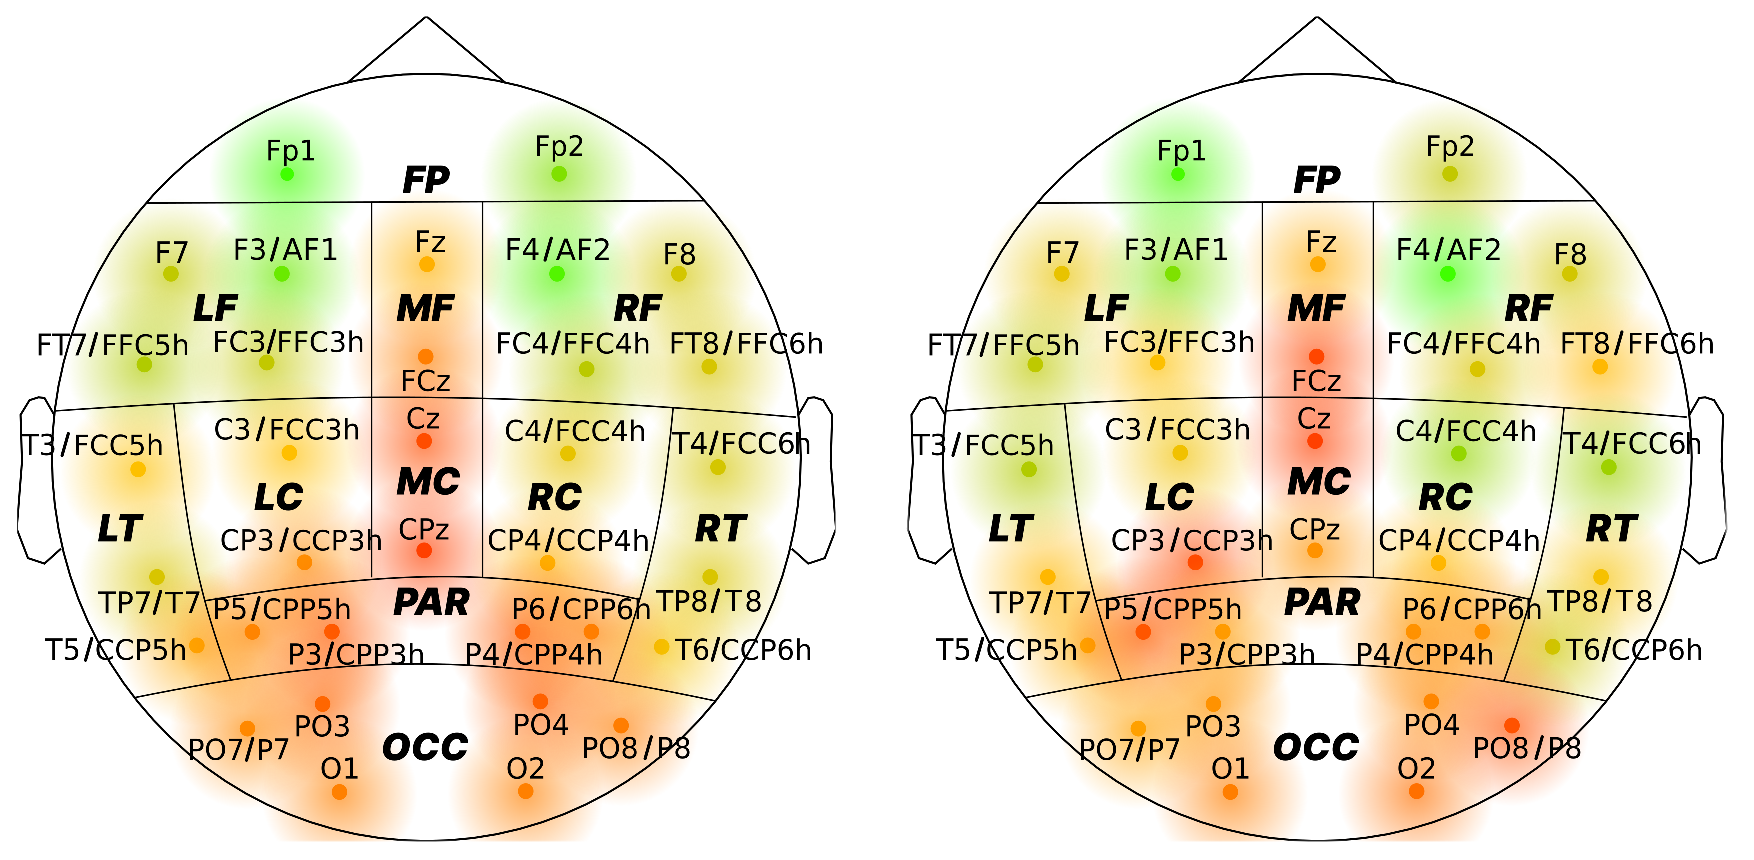
\includegraphics[width=0.58 \columnwidth]{Fig6.eps}
    \caption{Feature quality scores (QSDA on the left, IV on the right) aggregated by source electrode and averaged over 30 subjects. To account for the distinctions in electrode placement during different expeditions, we merge similar electrodes from different recordings into one point on the diagram. The respective mappings are indicated in the labels of such points using the `/' symbol}\label{figure6}
\end{figure}

Finally, the statistical analysis reveals that, on average, 27\% of topological features differ significantly between adjacent states in the original EEG, with none in the shuffled data. Consistent with the results of the first experiment, spectral validation in Table D2 shows comparably large statistics and pairwise significance for both feature sets. Together, these results support the robustness of the framework and indicate that topological features capture physiologically meaningful temporal structure.

Overall, the full-dataset results largely support the patterns observed in the initial analysis. Although some stage boundaries shifted when using topological features, main trends remained consistent, and robustness was supported by analyses of noisy and shuffled recordings. The proposed feature selection method also improved performance and was consistent with information values. Although further work is needed to clarify the physiological interpretation of the findings and the sources of the observed discrepancies, we believe that the framework is a viable alternative to spectral features.

\subsection{Sleep data}

To reinforce our results and evaluate the applicability of the topological approach to other data, we ran the proposed algorithm on PSG recordings from the Sleep-EDF~\cite{SleepEdf,PhysioNet} dataset. As mentioned previously, we search for 10 functional stages and estimate whether they fit any subset of expert annotations. For simplicity, this section analyzes three sets of features: spectral features similar to those in~\cite{SDA}, topological features, and a combination of both. Since the dataset contains only seven data channels, we omit feature selection. All hyperparameters of the algorithm were left unchanged.

For numerical expression of the results, we focus on two primary quality metrics: the previously used adapted silhouette score and the Fowlkes-Mallows index (FMI)~\cite{Fowlkes01091983}. The latter is a typical external criterion to measure the similarity between clusterings. For a predicted set of stage boundaries $A$ and an expert annotation $E$, we select a subset $F \subset E$ of boundaries with the lowest sum of pairwise distances to $A$: $\left( \sum_{i = 1}^{n} |a_i - f_i| \rightarrow \min \right)$ and compute the FMI to evaluate whether their `true' cluster distribution matches the predicted one. Although this matching procedure may lead to optimistic estimates, the comparison is intended to assess structural correspondence rather than provide an unbiased estimate of conventional sleep-staging accuracy.

To provide finer temporal granularity for boundary detection, we primarily focus on 15-second epochs, which are half of the conventional standard. This increases the number of observations per recording, provides SDA with a denser set of candidate transitions, and reduces the risk of boundaries being blurred by long averaging. The use of shorter epochs also highlights a potential advantage of the proposed framework for future high-resolution analyses, including sleep fragmentation and insomnia research.

As reported in Table~\ref{table2}, both epoch lengths yield qualitatively consistent results, with topological features retaining their substantial advantage in both metrics. For 15-second epochs, the adapted silhouette is seven times higher for topological features, whereas agreement with expert labels, measured by the FMI, averages 7\% better. With 30-second epochs, the advantage is smaller but remains consistent with conclusions.

\begin{table}[t]
\centering
\caption{Upper block: mean quality scores with 95\% confidence intervals for sleep data at two epoch lengths. Lower block: paired comparisons between topological and traditional features}\label{table2}
\begin{tabular}{lcccc}
  \toprule
    \multirow{2}{*}{Feature set / statistic} & \multicolumn{2}{c}{15-second epochs} & \multicolumn{2}{c}{30-second epochs} \\
     & Adapted silh. & FMI & Adapted silh. & FMI \\
  \midrule
    Traditional & $0.030 \pm 0.009$ & $0.843 \pm 0.017$ & $0.037 \pm 0.008$ & $0.834 \pm 0.017$ \\
    Topological & $0.228 \pm 0.010$ & $0.911 \pm 0.013$ & $0.191 \pm 0.009$ & $0.892 \pm 0.015$ \\
    Combined    & $0.227 \pm 0.010$ & $0.907 \pm 0.014$ & $0.185 \pm 0.009$ & $0.889 \pm 0.016$ \\
  \midrule
  \multicolumn{5}{l}{\textit{Paired comparison across subjects: topological ($B$) vs traditional ($A$), $H_1: B > A$}} \\
    Proportion $B > A$               & $0.987$                & $0.928$                & $0.993$ & $0.850$ \\
    Paired $t$ statistic             & $29.73$                & $14.79$                & $25.75$ & $12.66$ \\
    Paired $t$ $p$-value & $1.59 \times 10^{-65}$ & $1.51 \times 10^{-31}$ & $1.33 \times 10^{-57}$ & $7.52 \times 10^{-26}$ \\
    Wilcoxon $p$-value (one-sided) & $5.15 \times 10^{-25}$ & $4.07 \times 10^{-24}$ & $7.11 \times 10^{-26}$ & $1.09 \times 10^{-20}$ \\
    Cohen's $d_z$ & $2.403$ & $1.196$ & $2.082$ & $1.024$ \\
    Rank-biserial correlation & $0.957$ & $0.941$ & $0.974$ & $0.865$ \\
  \bottomrule
\end{tabular}
\end{table}

Unlike meditation experiment, a slightly lower performance of the combined feature space suggests that topological descriptors also capture most of the information provided by traditional techniques. Moreover, this observation is highly significant in both settings, as revealed in the lower block of Table~\ref{table2}: both the one-sided paired $t$-test and the Wilcoxon signed-rank test support superior quality of the topological approach, with large effect sizes and uniformly positive subject-level differences. The stronger result with shorter epochs is also consistent with finer temporal resolution and may reflect greater sensitivity to minor geometric changes in EEG structure.

Furthermore, Fig.~\ref{figure7} supports the physiological relevance of detected stages: those dominated by Wake epochs exhibit elevated power across all five frequency bands, with the largest values in higher-frequency, whereas N3-dominated stages show mildly reduced beta power, consistent with conventional interpretations of sleep phases. Importantly, the Kruskal---Wallis test confirms these differences are highly significant across all bands ($p < 10^{-4}$), suggesting that topological representation independently recovers interpretable signal structure without being explicitly designed to do so.

\begin{figure} 
    \centering 
    \begin{minipage}[t]{0.4\textwidth} 
        \vspace{0pt}
        \centering 
        
\includegraphics[width=\linewidth]{Fig7.eps} 
        \caption{Mean z-scored band power of TDA-detected stages grouped by dominant expert label, averaged over 153 subjects, with 95\% confidence intervals}\label{figure7} 
    \end{minipage} 
    \hfill 
    \begin{minipage}[t]{0.55\textwidth} 
        \vspace{0pt}
        \centering 
        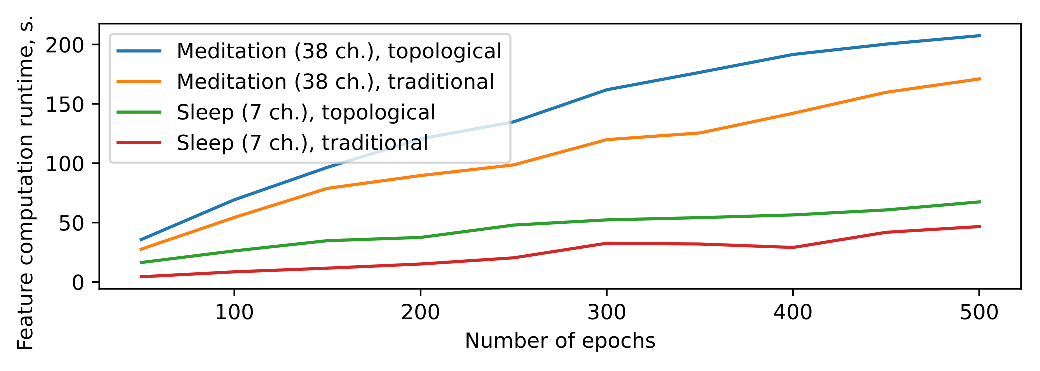
\includegraphics[width=\linewidth]{Fig8.eps}
        \caption{The running time in seconds for calculating traditional and topological features from EEG with varying numbers of epochs. Each point is an average of 25 measurements on a standard 8-core Intel Ice Lake VM with 16 GB of RAM.\@ The 95\% confidence intervals for each entry do not exceed 1\% of their value}\label{figure8} 
    \end{minipage} 
\end{figure}

Finally, Supplementary Materials E present comprehensive subject-wise results from the short-epoch experiment, indicating that all feature sets identified similar stages, with boundaries typically falling within compact groups of expert labels. The results signify that the algorithm captures reliable high-level structure despite the limit of 10 searched stages, and the scatter-plot densities further suggest that topological features yield more stable partitions that also align better with target annotations. 

Overall, the Sleep-EDF results are consistent with previous findings from meditation data and provide strong evidence supporting the topological approach. Despite limiting the search to ten stages, topological features consistently yielded more robust stages and better agreement with expert annotations, even without feature selection.

\section{Discussion}

In this study, we proposed a topological feature engineering pipeline for EEG segmentation, designed to capture its geometric and spatial structure. In the experiments, we established that the framework produced stages similar to those obtained with traditional features for Guhyasamaja Tantra meditation, and achieved substantially better agreement with expert annotations on the Sleep-EDF dataset. Robustness was further supported by noisy and shuffled data, as well as by statistical analyses, ablation, and physiological validation of spectral power. These findings extend previous applications of TDA in EEG studies, including ADHD classification~\cite{cai2024topologicalfeaturesearchmethod} and sleep staging~\cite{deng2024twostagehierarchicalexplainablefeature}, and establish that topological descriptors remain informative in unsupervised settings and compare favorably with state-of-the-art spectral features used in the field~\cite{SDA}.

Nonetheless, we suggest that neither approach extracts a complete description of the EEG in the general case. The benefit of combining topological and spectral features seems task-dependent: in some settings, the two provide complementary information, whereas in others topological features alone may be sufficient. Overall, these findings establish topological feature engineering as a viable and promising approach for EEG segmentation in the studied settings and motivate further validation.

Additionally, we introduced QSDA, an SDA-based feature selection framework designed for the full task and scalable to large feature sets. The experiments confirmed that QSDA effectively removed detrimental features, and its scores generally aligned with information values, a separate ranking procedure. Applied to Guhyasamaja Tantra meditation, QSDA identified frontal sensors as the primary source of informative features, an observation warranting further physiological investigation.

A major inherent limitation of QSDA is that both feature selection and evaluation rely on the same SDA objective. However, since the framework performs individual feature scoring rather than joint optimization, we believe the risk of circular bias is likely reduced, which is supported by the observed agreement with IV and other statistical tests. Nevertheless, nested evaluation on disjoint data partitions would provide stronger validation and is a worthwhile direction for future work.

Considering the huge dimensionality of the topological feature space, it is essential to assess whether presumed performance gains justify the added computational cost. Since the end-to-end runtime depends on several branches, a single informative closed-form expression of theoretical complexity is difficult to provide. We therefore conducted an empirical runtime analysis on samples from both datasets. As shown in Fig.~\ref{figure8}, topological features were indeed more expensive than traditional ones. In absolute terms, the topological pipeline for a typical complete meditation session of 1100 epochs required 11 minutes and 5 GB of RAM, compared to 5 minutes and 3 GB for the traditional approach. For a full night of sleep with over 2000 epochs, the corresponding runtimes were 19 and 7 minutes. The primary bottleneck of the topological approach, taking over 90\% of its runtime, was computing Vietoris---Rips complexes, whose worst-case complexity grows combinatorially with the number of points.

These results suggest that persistent homology may limit real-time use of the proposed framework, particularly for high-density EEG.\@ However, the additional cost relative to traditional features remains moderate, and there is substantial scope for optimization. Possible improvements include replacing Vietoris---Rips with faster constructions such as Alpha complexes and parallelizing the branches of the pipeline. Overall, the framework appears to be a practical alternative to traditional feature extraction, offering competitive performance at a reasonable computational cost.

Future work should evaluate the proposed approach on additional datasets to improve generalizability and identify recurring patterns. The consistently strong performance with 15-second epochs on the sleep dataset also suggests that the topological approach may be particularly beneficial for high-resolution analyses. A systematic comparison of epoch durations within the framework is therefore a natural next step, especially for clinical applications where fine-grained temporal precision may be critical. In addition, we anticipate valuable results from exploring the physiological implications of the patterns captured by topological features in light of existing domain knowledge, particularly considering the plausible association of the dimension-5 representative cocycles identified for subject~2 with the limbic system.

\section{Conclusion}

This study presents a feature engineering framework for time series data that serves as an effective alternative to spectral features for EEG segmentation with SDA, achieving comparable performance on two datasets. These results support the broader potential of topological feature engineering beyond EEG and motivate further work on its interpretability and physiological relevance. Additionally, we introduce QSDA, an SDA-based task-specific feature selection technique. Applied to meditation data, QSDA identified frontal electrodes as the main source of informative features, an observation that merits further investigation from a physiological perspective.

\section*{Declarations}

\subparagraph{\textbf{Data availability}}
Raw data will be made available by the authors upon request, without undue reservation. The source code supporting the experiments is located at https://github.com/TTPO100AJIEX/TopoEEG.

\subparagraph{\textbf{Ethics approval and consent to participate}}
The studies involving humans were approved by Moscow State University. The studies were conducted in accordance with the Declaration of Helsinki, the local legislation and institutional requirements. All participants provided written informed consent to participate in this study.

\subparagraph{\textbf{Competing interests}}
The authors declare no competing interests.

\subparagraph{\textbf{Acknowledgment}}
This study was supported by the Russian Science Foundation, Grant No. 24-68-00030.

\bibliography{references}

\subparagraph{\textbf{Aleksandr Abramov}} Data science and software engineering master's student at HSE University, Faculty of Computer Science.
\subparagraph{\textbf{Ekaterina Mikhaylets}} Associate professor at HSE University with a PhD in Discrete Mathematics and Mathematical Cybernetics.
\subparagraph{\textbf{Vsevolod Chernyshev}} Researcher at Ulm University with a PhD in Geometry and Topology.
\subparagraph{\textbf{Alexander Kaplan}} PhD and D.Sc in neurophysiology and psychophysiology from the Lomonosov Moscow State University, Professor and Head of the Laboratory for Neurophysiology and Neuro-Computer Interfaces.
\subparagraph{\textbf{Fedor Ratnikov}} PhD, associate professor at HSE University, Leading Researcher at the Laboratory of Methods for Big Data Analysis.

\end{document}
